


\tikzset{every picture/.style={line width=0.75pt}} %set default line width to 0.75pt        

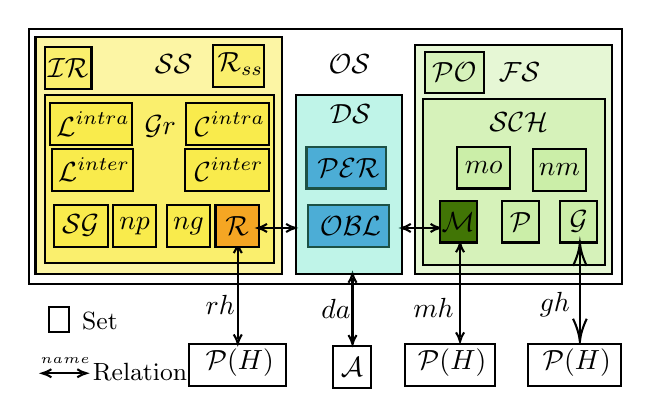
\begin{tikzpicture}[x=0.75pt,y=0.75pt,yscale=-1,xscale=1]
    %uncomment if require: \path (0,2218); %set diagram left start at 0, and has height of 2218

    %Shape: Rectangle [id:dp4397266155049817] 
    \draw  [fill={rgb, 255:red, 255; green, 255; blue, 255 }  ,fill opacity=1 ] (160,44) -- (446,44) -- (446,167) -- (160,167) -- cycle ;
    %Shape: Rectangle [id:dp6299944829788149] 
    \draw  [fill={rgb, 255:red, 184; green, 233; blue, 134 }  ,fill opacity=0.34 ] (346,52) -- (441.1,52) -- (441.1,162) -- (346,162) -- cycle ;
    %Shape: Rectangle [id:dp47821303258205083] 
    \draw  [fill={rgb, 255:red, 184; green, 233; blue, 134 }  ,fill opacity=0.34 ] (350,78) -- (437.83,78) -- (437.83,158) -- (350,158) -- cycle ;
    %Shape: Rectangle [id:dp23506628304013022] 
    \draw  [fill={rgb, 255:red, 248; green, 231; blue, 28 }  ,fill opacity=0.4 ] (163.27,48) -- (282,48) -- (282,162) -- (163.27,162) -- cycle ;
    %Straight Lines [id:da9243377050736461] 
    \draw    (367.82,149.31) -- (367.82,192.69) ;
    \draw [shift={(367.82,194.69)}, rotate = 270] [color={rgb, 255:red, 0; green, 0; blue, 0 }  ][line width=0.75]    (4.37,-1.96) .. controls (2.78,-0.92) and (1.32,-0.27) .. (0,0) .. controls (1.32,0.27) and (2.78,0.92) .. (4.37,1.96)   ;
    \draw [shift={(367.82,147.31)}, rotate = 90] [color={rgb, 255:red, 0; green, 0; blue, 0 }  ][line width=0.75]    (4.37,-1.96) .. controls (2.78,-0.92) and (1.32,-0.27) .. (0,0) .. controls (1.32,0.27) and (2.78,0.92) .. (4.37,1.96)   ;
    %Straight Lines [id:da07842537976091113] 
    \draw    (341.69,140) -- (356,140) ;
    \draw [shift={(358,140)}, rotate = 180] [color={rgb, 255:red, 0; green, 0; blue, 0 }  ][line width=0.75]    (4.37,-1.96) .. controls (2.78,-0.92) and (1.32,-0.27) .. (0,0) .. controls (1.32,0.27) and (2.78,0.92) .. (4.37,1.96)   ;
    \draw [shift={(339.69,140)}, rotate = 0] [color={rgb, 255:red, 0; green, 0; blue, 0 }  ][line width=0.75]    (4.37,-1.96) .. controls (2.78,-0.92) and (1.32,-0.27) .. (0,0) .. controls (1.32,0.27) and (2.78,0.92) .. (4.37,1.96)   ;
    %Shape: Rectangle [id:dp5703456898638302] 
    \draw  [fill={rgb, 255:red, 248; green, 231; blue, 28 }  ,fill opacity=0.4 ] (167.81,76) -- (278,76) -- (278,157) -- (167.81,157) -- cycle ;
    %Shape: Rectangle [id:dp6202366628126772] 
    \draw  [fill={rgb, 255:red, 255; green, 255; blue, 255 }  ,fill opacity=1 ] (341.12,196) -- (384.8,196) -- (384.8,216) -- (341.12,216) -- cycle ;

    %Shape: Rectangle [id:dp20067598884831228] 
    \draw  [fill={rgb, 255:red, 248; green, 231; blue, 28 }  ,fill opacity=0.4 ] (200.59,129) -- (221.41,129) -- (221.41,149) -- (200.59,149) -- cycle ;

    %Shape: Rectangle [id:dp5229429696525485] 
    \draw  [fill={rgb, 255:red, 248; green, 231; blue, 28 }  ,fill opacity=0.4 ] (172,129) -- (198,129) -- (198,149) -- (172,149) -- cycle ;
    %Shape: Rectangle [id:dp92237875722883] 
    \draw  [fill={rgb, 255:red, 248; green, 231; blue, 28 }  ,fill opacity=0.4 ] (171.02,102) -- (210.03,102) -- (210.03,122) -- (171.02,122) -- cycle ;

    %Shape: Rectangle [id:dp6591761395302378] 
    \draw  [fill={rgb, 255:red, 248; green, 231; blue, 28 }  ,fill opacity=0.4 ] (170.22,80) -- (209.8,80) -- (209.8,100) -- (170.22,100) -- cycle ;

    %Shape: Rectangle [id:dp11794703752595392] 
    \draw  [fill={rgb, 255:red, 248; green, 231; blue, 28 }  ,fill opacity=0.4 ] (235.83,80) -- (275.95,80) -- (275.95,100) -- (235.83,100) -- cycle ;

    %Shape: Rectangle [id:dp6557958558103134] 
    \draw  [fill={rgb, 255:red, 248; green, 231; blue, 28 }  ,fill opacity=0.4 ] (235.29,102) -- (275.72,102) -- (275.72,122) -- (235.29,122) -- cycle ;

    %Shape: Rectangle [id:dp8284992701408749] 
    \draw  [fill={rgb, 255:red, 65; green, 117; blue, 5 }  ,fill opacity=1 ] (358.01,127) -- (375.99,127) -- (375.99,147) -- (358.01,147) -- cycle ;

    %Shape: Rectangle [id:dp7066110016250453] 
    \draw  [fill={rgb, 255:red, 248; green, 231; blue, 28 }  ,fill opacity=0.4 ] (226.63,129) -- (247.37,129) -- (247.37,149) -- (226.63,149) -- cycle ;

    %Shape: Rectangle [id:dp4021333114319714] 
    \draw  [fill={rgb, 255:red, 248; green, 231; blue, 28 }  ,fill opacity=0.4 ] (167.75,53) -- (190.25,53) -- (190.25,73) -- (167.75,73) -- cycle ;

    %Shape: Rectangle [id:dp8476756388266236] 
    \draw  [fill={rgb, 255:red, 248; green, 231; blue, 28 }  ,fill opacity=0.4 ] (248.98,52) -- (273.16,52) -- (273.16,72) -- (248.98,72) -- cycle ;

    %Shape: Rectangle [id:dp07470576340681823] 
    \draw  [fill={rgb, 255:red, 74; green, 144; blue, 226 }  ,fill opacity=1 ] (293.84,101) -- (332.24,101) -- (332.24,121) -- (293.84,121) -- cycle ;

    %Shape: Rectangle [id:dp31407652093057714] 
    \draw  [fill={rgb, 255:red, 74; green, 144; blue, 226 }  ,fill opacity=1 ] (294.57,129) -- (333.48,129) -- (333.48,149) -- (294.57,149) -- cycle ;

    %Shape: Rectangle [id:dp053729126169398844] 
    \draw  [fill={rgb, 255:red, 184; green, 233; blue, 134 }  ,fill opacity=0.34 ] (350.75,55) -- (379.25,55) -- (379.25,75) -- (350.75,75) -- cycle ;

    %Shape: Rectangle [id:dp7720103442630182] 
    \draw  [fill={rgb, 255:red, 184; green, 233; blue, 134 }  ,fill opacity=0.34 ] (366.43,101) -- (392,101) -- (392,121) -- (366.43,121) -- cycle ;

    %Shape: Rectangle [id:dp3183552657000306] 
    \draw  [fill={rgb, 255:red, 184; green, 233; blue, 134 }  ,fill opacity=0.34 ] (403.11,102) -- (428.29,102) -- (428.29,122) -- (403.11,122) -- cycle ;

    %Shape: Rectangle [id:dp10802424702469593] 
    \draw  [fill={rgb, 255:red, 184; green, 233; blue, 134 }  ,fill opacity=0.34 ] (416.02,127) -- (434,127) -- (434,147) -- (416.02,147) -- cycle ;

    %Shape: Rectangle [id:dp16589412198505937] 
    \draw  [fill={rgb, 255:red, 184; green, 233; blue, 134 }  ,fill opacity=0.34 ] (388,127) -- (405.98,127) -- (405.98,147) -- (388,147) -- cycle ;

    %Shape: Rectangle [id:dp1270989692188249] 
    \draw  [fill={rgb, 255:red, 255; green, 255; blue, 255 }  ,fill opacity=1 ] (237.2,196) -- (284,196) -- (284,216) -- (237.2,216) -- cycle ;

    %Straight Lines [id:da6196983489979997] 
    \draw    (260.73,149.69) -- (260.73,193.69) ;
    \draw [shift={(260.73,195.69)}, rotate = 270] [color={rgb, 255:red, 0; green, 0; blue, 0 }  ][line width=0.75]    (4.37,-1.96) .. controls (2.78,-0.92) and (1.32,-0.27) .. (0,0) .. controls (1.32,0.27) and (2.78,0.92) .. (4.37,1.96)   ;
    \draw [shift={(260.73,147.69)}, rotate = 90] [color={rgb, 255:red, 0; green, 0; blue, 0 }  ][line width=0.75]    (4.37,-1.96) .. controls (2.78,-0.92) and (1.32,-0.27) .. (0,0) .. controls (1.32,0.27) and (2.78,0.92) .. (4.37,1.96)   ;
    %Shape: Rectangle [id:dp21027747628033966] 
    \draw  [fill={rgb, 255:red, 245; green, 166; blue, 35 }  ,fill opacity=1 ] (250,129) -- (270.77,129) -- (270.77,149) -- (250,149) -- cycle ;

    %Shape: Rectangle [id:dp3309840870842591] 
    \draw  [fill={rgb, 255:red, 255; green, 255; blue, 255 }  ,fill opacity=1 ] (169.81,178) -- (179.61,178) -- (179.61,190) -- (169.81,190) -- cycle ;
    %Straight Lines [id:da9379387705027007] 
    \draw    (168.54,210) -- (185.78,210) ;
    \draw [shift={(187.78,210)}, rotate = 180] [color={rgb, 255:red, 0; green, 0; blue, 0 }  ][line width=0.75]    (4.37,-1.96) .. controls (2.78,-0.92) and (1.32,-0.27) .. (0,0) .. controls (1.32,0.27) and (2.78,0.92) .. (4.37,1.96)   ;
    \draw [shift={(166.54,210)}, rotate = 0] [color={rgb, 255:red, 0; green, 0; blue, 0 }  ][line width=0.75]    (4.37,-1.96) .. controls (2.78,-0.92) and (1.32,-0.27) .. (0,0) .. controls (1.32,0.27) and (2.78,0.92) .. (4.37,1.96)   ;
    %Shape: Rectangle [id:dp07012270906311535] 
    \draw  [fill={rgb, 255:red, 255; green, 255; blue, 255 }  ,fill opacity=1 ] (306.78,197) -- (324.75,197) -- (324.75,217) -- (306.78,217) -- cycle ;

    %Straight Lines [id:da20015846115702463] 
    \draw    (316,164) -- (316,194) ;
    \draw [shift={(316,196)}, rotate = 270] [color={rgb, 255:red, 0; green, 0; blue, 0 }  ][line width=0.75]    (4.37,-1.96) .. controls (2.78,-0.92) and (1.32,-0.27) .. (0,0) .. controls (1.32,0.27) and (2.78,0.92) .. (4.37,1.96)   ;
    \draw [shift={(316,162)}, rotate = 90] [color={rgb, 255:red, 0; green, 0; blue, 0 }  ][line width=0.75]    (4.37,-1.96) .. controls (2.78,-0.92) and (1.32,-0.27) .. (0,0) .. controls (1.32,0.27) and (2.78,0.92) .. (4.37,1.96)   ;
    %Straight Lines [id:da22484911594965085] 
    \draw    (286.4,140) -- (272.42,140) ;
    \draw [shift={(270.42,140)}, rotate = 360] [color={rgb, 255:red, 0; green, 0; blue, 0 }  ][line width=0.75]    (4.37,-1.96) .. controls (2.78,-0.92) and (1.32,-0.27) .. (0,0) .. controls (1.32,0.27) and (2.78,0.92) .. (4.37,1.96)   ;
    \draw [shift={(288.4,140)}, rotate = 180] [color={rgb, 255:red, 0; green, 0; blue, 0 }  ][line width=0.75]    (4.37,-1.96) .. controls (2.78,-0.92) and (1.32,-0.27) .. (0,0) .. controls (1.32,0.27) and (2.78,0.92) .. (4.37,1.96)   ;
    %Shape: Rectangle [id:dp9631304723399212] 
    \draw  [fill={rgb, 255:red, 80; green, 227; blue, 194 }  ,fill opacity=0.36 ] (288.57,76) -- (340,76) -- (340,162) -- (288.57,162) -- cycle ;
    %Straight Lines [id:da6995772701176901] 
    \draw    (425.55,149.31) -- (425.55,192.69) ;
    \draw [shift={(425.55,194.69)}, rotate = 270] [color={rgb, 255:red, 0; green, 0; blue, 0 }  ][line width=0.75]    (10.93,-3.29) .. controls (6.95,-1.4) and (3.31,-0.3) .. (0,0) .. controls (3.31,0.3) and (6.95,1.4) .. (10.93,3.29)   ;
    \draw [shift={(425.55,147.31)}, rotate = 90] [color={rgb, 255:red, 0; green, 0; blue, 0 }  ][line width=0.75]    (10.93,-3.29) .. controls (6.95,-1.4) and (3.31,-0.3) .. (0,0) .. controls (3.31,0.3) and (6.95,1.4) .. (10.93,3.29)   ;
    %Shape: Rectangle [id:dp7604827971406838] 
    \draw  [fill={rgb, 255:red, 255; green, 255; blue, 255 }  ,fill opacity=1 ] (400.41,196) -- (445.45,196) -- (445.45,216) -- (400.41,216) -- cycle ;



    % Text Node
    \draw (413.5,177) node   [align=left] {$\displaystyle gh$};
    % Text Node
    \draw (177.57,204) node  [font=\tiny] [align=left] {$\displaystyle name$};
    % Text Node
    \draw (308,179) node   [align=left] {$\displaystyle da$};
    % Text Node
    \draw (210.66,207) node  [font=\footnotesize] [align=left] {\begin{minipage}[lt]{29.67pt}\setlength\topsep{0pt}
            \begin{center}
                {\small Relation}
            \end{center}

        \end{minipage}};
    % Text Node
    \draw (194.32,185) node  [font=\footnotesize] [align=left] {\begin{minipage}[lt]{13.75pt}\setlength\topsep{0pt}
            \begin{center}
                {\small Set}
            \end{center}

        \end{minipage}};
    % Text Node
    \draw (314.5,61) node   [align=left] {$\displaystyle \mathcal{OS}$};
    % Text Node
    \draw (185,139) node   [align=left] {$\displaystyle \mathcal{SG}$};
    % Text Node
    \draw (315,85) node   [align=left] {$\displaystyle \mathcal{DS}$};
    % Text Node
    \draw (229.87,61) node   [align=left] {$\displaystyle \mathcal{SS}$};
    % Text Node
    \draw (355,178.31) node   [align=left] {$\displaystyle mh$};
    % Text Node
    \draw (252.32,177) node   [align=left] {$\displaystyle rh$};
    % Text Node
    \draw (223.38,91) node   [align=left] {$\displaystyle \mathcal{G}r$};
    % Text Node
    \draw (396.5,65) node   [align=left] {$\displaystyle \mathcal{FS}$};
    % Text Node
    \draw (396.04,89) node   [align=left] {$\displaystyle \mathcal{SCH}$};
    % Text Node
    \draw (424,205) node   [align=left] {$\displaystyle \mathcal{P}(H)$};
    % Text Node
    \draw (315.76,207) node   [align=left] {$\displaystyle \mathcal{A}$};
    % Text Node
    \draw (260.38,139) node   [align=left] {$\displaystyle \mathcal{R}$};
    % Text Node
    \draw (261.71,205) node   [align=left] {$\displaystyle \mathcal{P}(H)$};
    % Text Node
    \draw (396.99,137) node   [align=left] {$\displaystyle \mathcal{P}$};
    % Text Node
    \draw (425.01,137) node   [align=left] {$\displaystyle \mathcal{G}$};
    % Text Node
    \draw (415.7,112) node   [align=left] {$\displaystyle nm$};
    % Text Node
    \draw (379.21,111) node   [align=left] {$\displaystyle mo$};
    % Text Node
    \draw (365,65) node   [align=left] {$\displaystyle \mathcal{PO}$};
    % Text Node
    \draw (315,139) node   [align=left] {$\displaystyle \mathcal{OBL}$};
    % Text Node
    \draw (314,111) node   [align=left] {$\displaystyle \mathcal{PER}$};
    % Text Node
    \draw (262,61) node   [align=left] {$\displaystyle \mathcal{R}_{ss}$};
    % Text Node
    \draw (179,63) node   [align=left] {$\displaystyle \mathcal{IR}$};
    % Text Node
    \draw (237,139) node   [align=left] {$\displaystyle ng$};
    % Text Node
    \draw (367,137) node   [align=left] {$\displaystyle \mathcal{M}$};
    % Text Node
    \draw (256.51,112) node   [align=left] {$\displaystyle \mathcal{C}^{inter}$};
    % Text Node
    \draw (256.89,90) node   [align=left] {$\displaystyle \mathcal{C}^{intra}$};
    % Text Node
    \draw (191,90) node   [align=left] {$\displaystyle \mathcal{L}^{intra}$};
    % Text Node
    \draw (191.5,112) node   [align=left] {$\displaystyle \mathcal{L}^{inter}$};
    % Text Node
    \draw (211,139) node   [align=left] {$\displaystyle np$};
    % Text Node
    \draw (364,205) node   [align=left] {$\displaystyle \mathcal{P}(H)$};


\end{tikzpicture}